\section{From forecast uncertainty to a certified position change}
\label{sec:certifiedposition}

An interval can support two different objectives: minimizing worst-case
regret to an oracle, as in Section~\ref{sec:intervalposition}, or maximizing
a guaranteed improvement over a specified baseline. The latter is useful
when the alternative is to retain an existing holding. The two objectives
should not be conflated. Robust trading and convex cost-aware allocation
are established methods \citep{BoydEtAl2017}; the contribution here is an
explicit connection between a forecast set, a baseline-relative no-trade
region, and a sequential certificate for realized decision outcomes.

\subsection{A multi-asset improvement objective}

At a decision time, all of the following quantities are measurable using
the trader's available information. Let $K$ be a nonempty compact convex
set, $b\in K$ a baseline position, and $F$ a finite continuous convex
cost-and-risk function on $K$. Suppose the conditional mean return lies in
\[
 \mathcal U=m+\{Sv:\|v\|_2\le\rho\},\qquad \rho\ge0.
\]
For $w\in K$ define the worst-case conditional improvement
\begin{equation}\label{eq:robustpositiongain}
 G(w;b)=m^\top(w-b)-\rho\|S^\top(w-b)\|_2-F(w)+F(b).
\end{equation}
The uncertainty is in the conditional mean, not in an individual realized
return. A prediction interval for the next noisy return is not automatically
a confidence set for its conditional mean.

\begin{theorem}[Baseline-relative position certificate]
\label{thm:robustpositiongain}
For every $w\in K$,
\[
 G(w;b)=\inf_{\mu\in\mathcal U}
 \{\mu^\top(w-b)-F(w)+F(b)\}.
\]
It is a continuous concave function with $G(b;b)=0$. A maximizer $w_R$
exists and guarantees conditional objective improvement at least
$G(w_R;b)\ge0$ for every $\mu\in\mathcal U$. If $F$ is $a$-strongly
convex, $a>0$, the maximizer is unique and
\begin{equation}\label{eq:positiondistancegain}
 G(w_R;b)\ge\tfrac a2\|w_R-b\|_2^2.
\end{equation}
An approximate solution with certified lower improvement $g\ge0$ retains
the guarantee $g$; a negative or unresolved lower bound triggers $b$.
\end{theorem}
\begin{proof}
The support function of the Euclidean ball gives the displayed infimum.
Concavity, continuity and compactness prove attainment. The feasible
baseline proves nonnegative optimal value. Strong convexity of $F$ makes
$-G$ strongly convex and gives uniqueness. At its constrained minimum,
the strong-convexity variational inequality gives
$-G(b;b)\ge-G(w_R;b)+a\|b-w_R\|^2/2$, which proves
\eqref{eq:positiondistancegain}. The final claim is the definition of a
valid lower bound on $G$.
\end{proof}

\begin{proposition}[The portfolio no-trade region]
\label{prop:portfolionotrade}
Let
$F(w)=\tfrac12w^\top Hw+\sum_i c_i|w_i-b_i|$, where $H\succ0$ and
$c_i\ge0$. With the normal cone
$N_K(b)=\{n:n^\top(w-b)\le0\text{ for all }w\in K\}$,
the baseline is optimal if and only if
\begin{equation}\label{eq:portfolionotrade}
 m-Hb\in
 \prod_i[-c_i,c_i]+\{Sv:\|v\|_2\le\rho\}+N_K(b).
\end{equation}
For one asset, mean interval $[m-e,m+e]$, quadratic coefficient $a>0$,
proportional cost $c\ge0$ and feasible interval $K=[L,U]$ containing $b$,
\begin{equation}\label{eq:robustsoft}
 w_R=b+\operatorname{clip}_{[L-b,U-b]}
       \left(\frac{\soft_{c+e}(m-ab)}{a}\right).
\end{equation}
Without an active position cap the guaranteed improvement is
$(|m-ab|-c-e)_+^2/(2a)$.
\end{proposition}
\begin{proof}
The subgradient of the proportional term at $b$ is the displayed box.
The subgradient at zero of $\rho\|S^\top d\|$ is the image of the radius
$\rho$ ball under $S$. The constrained convex optimality condition is
therefore precisely \eqref{eq:portfolionotrade}; the norm and cost terms
are finite and continuous, so the usual subgradient sum rule applies.
In one dimension, writing $d=w-b$ reduces the objective to
$(m-ab)d-a d^2/2-(c+e)|d|$. Its maximizer is the stated soft threshold,
clipped to the feasible interval. Substitution proves the value formula.
\end{proof}

The current inventory enters through $ab$, trading cost through $c$, and
forecast uncertainty through $e$. A high raw forecast need not justify a
trade when inventory is already large. Uncertainty enlarges the no-trade
region by an economically interpretable amount. The formula starts from
the inherited holding $b$; if a comparator differs from that holding, the
transaction-cost difference must be recomputed for both alternatives.

\subsection{A time-uniform realized-outcome certificate}

Conditional expected improvement and realized performance are different.
The following transfer keeps that distinction explicit. Index nonoverlapping
evaluation periods by $t=1,2,\ldots$, with decisions measurable in
$\mathcal F_{t-1}$ and observed returns $R_t$. Let $w_t,b_t$ be predictable
positions, $d_t=w_t-b_t$, and $k_t$ the predictable difference of their
declared cost-and-risk charges. For two separately evolving strategies,
compute each charge using its own inherited inventory and actual modeled
turnover. Put
\[
 \mu_t=\E[R_t\mid\mathcal F_{t-1}],\quad
 Y_t=d_t^\top R_t-k_t,\quad
 h_t=d_t^\top\mu_t-k_t.
\]
$Y_t$ is realized net return difference if the charges are monetary costs;
when they include risk penalties, it is a realized penalized objective,
not cash P\&L. Suppose predictable numbers $g_t$ satisfy
\begin{equation}\label{eq:coverageevent}
 \Pr\{h_t\ge g_t\text{ for every }t\}\ge1-\delta.
\end{equation}
Simultaneously valid conditional-mean sets and exact cost differences
provide one route to this event. Suppose also that for every real $\lambda$
the residual $\xi_t=d_t^\top(R_t-\mu_t)$ obeys
\begin{equation}\label{eq:predictablesubgaussian}
 \E[\exp(\lambda\xi_t)\mid\mathcal F_{t-1}]
       \le\exp(\lambda^2v_t/2),
\end{equation}
where $v_t\ge0$ is predictable. This is a conditional tail assumption,
not a conclusion from an unconditional variance estimate.

\begin{theorem}[Sequential transfer of certified improvement]
\label{thm:sequentialgain}
Let $V_n=\sum_{t\le n}v_t$, fix $v_0>0$ and $0<\alpha<1$ in advance,
and define
\begin{equation}\label{eq:mixtureboundary}
 B_\alpha(V)=
 \sqrt{(V+v_0)\log\!\left(\frac{V+v_0}{v_0\alpha^2}\right)}.
\end{equation}
Under \eqref{eq:coverageevent}--\eqref{eq:predictablesubgaussian}, with
probability at least $1-\delta-\alpha$, simultaneously for every $n\ge1$,
\begin{equation}\label{eq:realizedgain}
 \sum_{t\le n}Y_t\ge\sum_{t\le n}g_t-B_\alpha(V_n).
\end{equation}
The same event covers any data-dependent stopping time.
\end{theorem}
\begin{proof}
For each fixed $\lambda\in\R$, conditional iteration makes
$\exp(\lambda\sum_{t\le n}\xi_t-\lambda^2 V_n/2)$ a nonnegative
supermartingale starting at one. Mix it against a normal distribution
of $\lambda$ with mean zero and variance $1/v_0$. Tonelli's theorem and
the Gaussian integral give the nonnegative supermartingale
\[
 Z_n=\sqrt{\frac{v_0}{v_0+V_n}}
       \exp\!\left(\frac{(\sum_{t\le n}\xi_t)^2}{2(v_0+V_n)}\right).
\]
Ville's inequality bounds $\Pr\{\sup_n Z_n\ge1/\alpha\}$ by $\alpha$.
Solving this threshold gives
$|\sum_{t\le n}\xi_t|\le B_\alpha(V_n)$ at every $n$ outside that event.
Intersect with \eqref{eq:coverageevent}, use the union bound, and sum
$Y_t=h_t+\xi_t$. Uniformity in $n$ implies the stopping-time statement.
\end{proof}

\begin{remark}\label{rem:sequential-general}
The proof of Theorem~\ref{thm:sequentialgain} uses the form
$Y_t=d_t^\top R_t-k_t$ only through the decomposition $Y_t=h_t+\xi_t$ with
$h_t$ predictable. It therefore applies to any settled per-period outcome whose
centered part $\xi_t=Y_t-\mathbb E[Y_t\mid\mathcal F_{t-1}]$ satisfies \eqref{eq:predictablesubgaussian}.
\end{remark}

This is a normal-mixture confidence-sequence argument, specialized to
predictable position differences; the general methodology is developed
by \citet{HowardEtAl2021}. It does not require independent returns.
It does require the stated conditional moment bound and correct predictable
cost accounting. A negative lower bound is inconclusive. Selecting a favorable
fixed-time confidence interval after repeatedly inspecting P\&L is not a
substitute for \eqref{eq:realizedgain}.

\begin{corollary}[From event history to a realized outcome]\label{cor:main-chain}
Consider nonoverlapping periods $t=1,2,\dots$, with $R_t$ the reference-price
increment over period $t$ and $\mathcal F_{t-1}$ the trader's information at its
start. At each $t$ apply Theorem~\ref{thm:eventinterval} with forecast
horizon equal to the period length, and assume its history-likelihood lower
bound is positive; write $[l_t,u_t]$ for the resulting interval. Let $E$ be the
event that the primitive enclosures used there contain the true generator,
marks and prior at every $t$, and suppose $\Pr(E)\ge1-\delta$. Let $a_t>0$, $c_t\ge0$ and the endpoints of a compact feasible interval
$K_t$ containing the inherited holding $b_t$ be predictable. Use
$F_t(w)=a_tw^2/2+c_t|w-b_t|$. At each time, choose $w_t$ by \eqref{eq:robustsoft} with $a=a_t$, $c=c_t$, $K=K_t$, $m=(l_t+u_t)/2$ and $e=(u_t-l_t)/2$,
let $k_t=F_t(w_t)-F_t(b_t)$ be its declared charge, and let
$g_t=G_t(w_t;b_t)$ be its guaranteed improvement, where $G_t$ is
\eqref{eq:robustpositiongain} with the time-$t$ inputs. Set $Y_t=(w_t-b_t)R_t-k_t$ and $\mu_t=\E[R_t\mid\mathcal F_{t-1}]$. If
$\xi_t=(w_t-b_t)(R_t-\mu_t)$ satisfies \eqref{eq:predictablesubgaussian}, then with probability at least
$1-\delta-\alpha$, simultaneously for all $n\ge1$,
\[
  \sum_{t\le n}Y_t\ \ge\ \sum_{t\le n}g_t-B_\alpha(V_n).
\]
\end{corollary}

\begin{proof}
On $E$, Theorem~\ref{thm:eventinterval} gives
$\mu_t=\mathbb E[R_t\mid\mathcal F_{t-1}]\in[l_t,u_t]$. This interval is the set
$U$ of Theorem~\ref{thm:robustpositiongain} with $S=e$ and $\rho=1$, so
$h_t=\mu_t(w_t-b_t)-k_t\ge G_t(w_t;b_t)=g_t$ for every $t$ on $E$, which is
condition~\eqref{eq:coverageevent}. Theorem~\ref{thm:sequentialgain} completes the proof.
\end{proof}
If the model is time-homogeneous and the enclosure box is fixed, $E$ is the
single event that the box contains the true parameter. For a box constructed
from a calibration sample independent of the deployment period,
$\Pr$ refers to their joint law.

\subsection{What calibration must supply}

Equation~\eqref{eq:coverageevent} requires simultaneous coverage along the
deployment path. Fixed-time intervals with nominal coverage $1-\delta$ at
each time do not imply it. One elementary construction assigns levels
$\delta_t>0$ with $\sum_t\delta_t\le\delta$ and proves marginal coverage
for each time; a union bound then suffices without independence. Properly
constructed confidence sequences can be less conservative. Neither route
turns ordinary conformal coverage for noisy returns into conditional-mean
coverage without an additional argument.

Model uncertainty, return noise, and unobserved execution cost are separate
budgets. The theorem uses the first through $g_t$, the second through $V_n$,
and assumes the cost difference is already known predictably. Random slippage
or fills must instead enter the realized outcome and its conditional residual,
with a corresponding mean enclosure and moment bound. Latency must be
included when forming the information set. Overlapping return horizons
cannot be inserted as if their realized labels arrive before each next
decision. Finally, repeated one-step decisions relative to the current
holding compare with a sequence of local alternatives; they are not by
themselves a global guarantee against a separately evolving baseline policy.

\subsection{Reproducible position and sequential experiments}

The script \texttt{verification/certified\_improvement.py} independently
checks scalar clipped decisions with bounded minimization, portfolio
support values with a constrained optimizer, and the Gaussian-mixture
integral with numerical quadrature. It then simulates a declared Gaussian
return model with predictable positions, valid deterministic mean
enclosures, and known conditional noise scale. The table reports exact
one-period robust decisions for $m=0.12$, $a=1$, $c=0.02$, $b=0$ and
$|w|\le0.20$.

\begin{table}[htbp]
\centering
\caption{Synthetic scalar forecast experiment. Increasing conditional-mean
uncertainty can turn a positive forecast into a no-trade decision.}
\label{tab:certifiedposition}
\begin{tabular}{rrrr}
\toprule
Mean radius & Nominal position & Robust position & Guaranteed gain\\
\midrule
\inputtable{tables/certified_improvement_rows.tex}
\bottomrule
\end{tabular}
\end{table}

\begin{figure}[htbp]
\centering
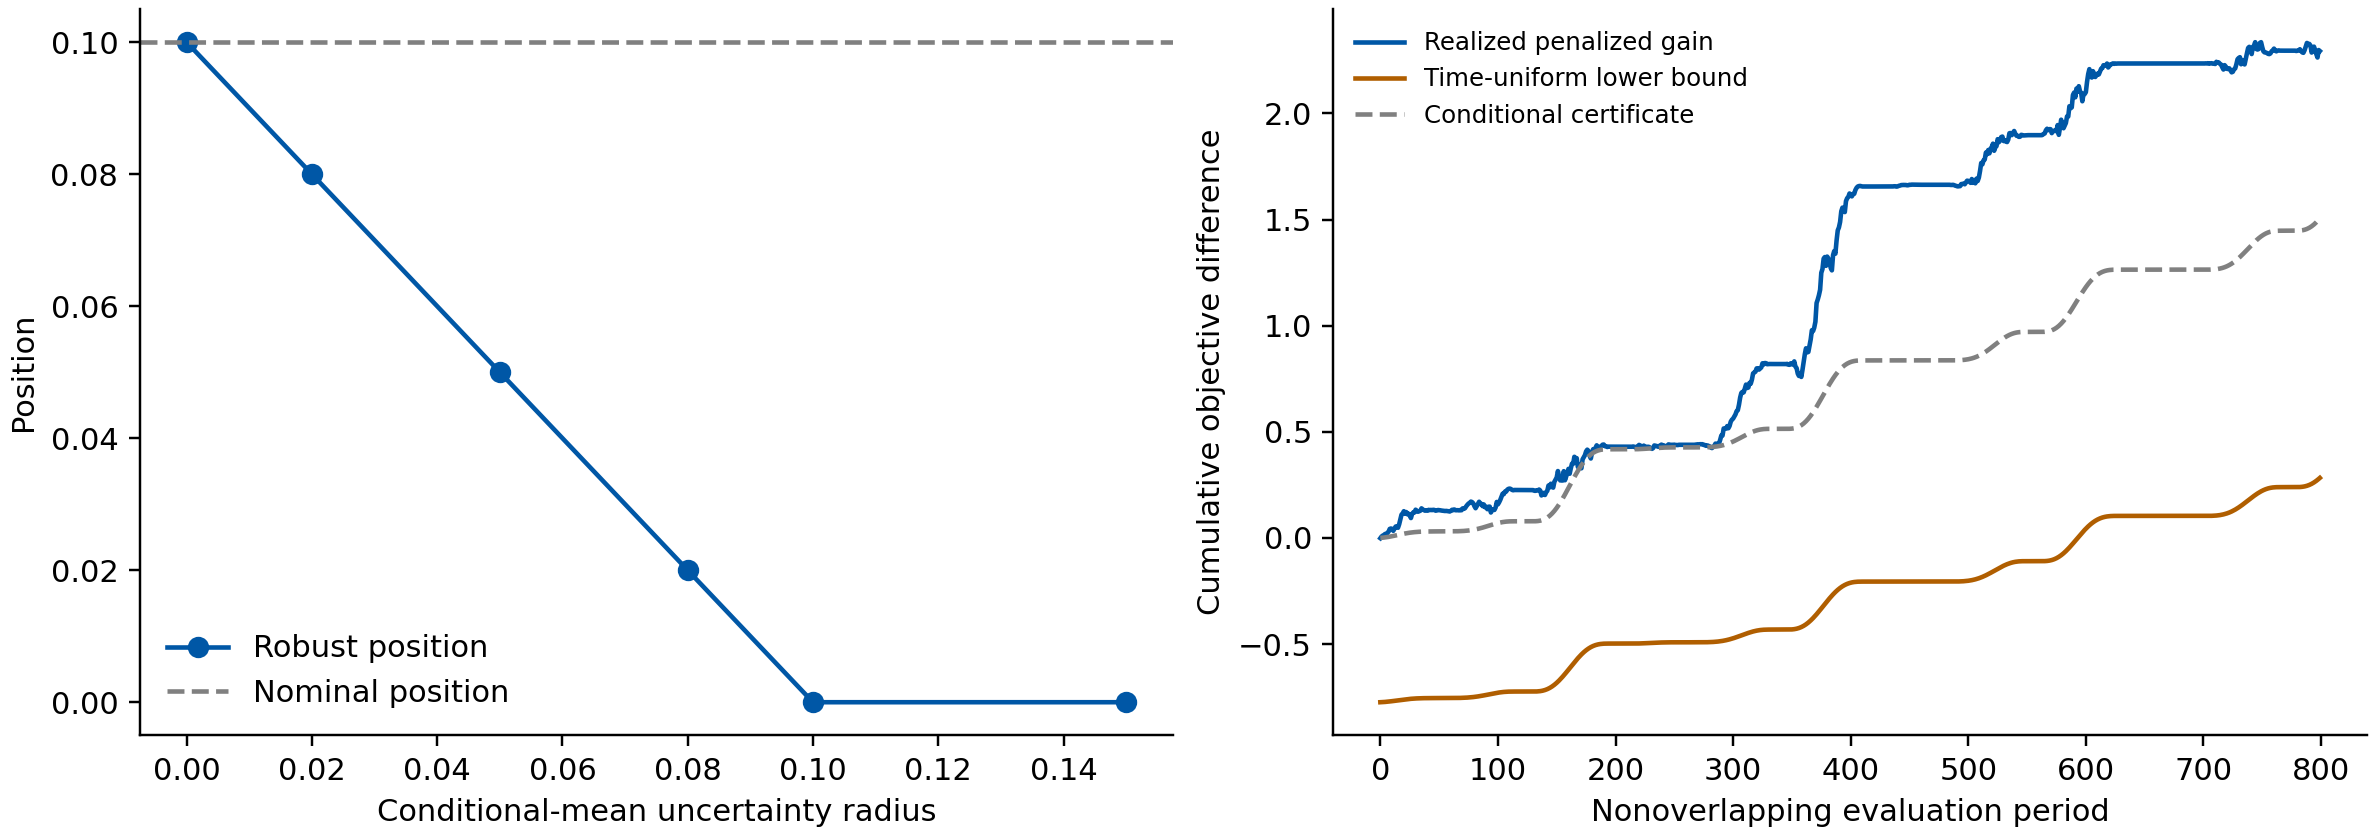
\includegraphics[width=0.94\linewidth]{figures/06_certified_improvement.png}
\caption{Uncertainty-aware position sizing and a realized sequential
objective. The lower curve is the cumulative conditional certificate minus
the time-uniform noise allowance, not a guaranteed positive P\&L curve.
All paths and forecasts are synthetic.}
\end{figure}

The saved report includes the seed, horizon, noise scale, boundary level,
cumulative conditional certificate, realized objective, and observed
boundary crossings across repeated simulations. The simulation is a
diagnostic of the implementation; the theorem supplies the probability
guarantee. A market evaluation must additionally establish coverage,
conditional tails, timestamp causality and the costs of the executable
position changes. None is inferred from the synthetic pass rate.
